\lstdefinelanguage{ST}{
        keywords={FUNCTION_BLOCK,VAR_INPUT,END_VAR,VAR_OUTPUT,VAR,NOT,IF,END_IF,THEN,ELSE,PROGRAM},
        morekeywords={TRUE,FALSE},
		sensitive=true,%
%		alsoletter={\$},%
%		comment=[l]{t\#},%
}
\lstset{language=ST,
        basicstyle=\footnotesize\ttfamily,
        breaklines=true,
        tabsize=2,
        numbers=left,
        numberstyle=\tiny,
        numbersep=7pt,
        showspaces=false,
        keywordstyle=\color{blue}\textbf,       
        commentstyle=\color{magenta},
        showstringspaces=false,
        stringstyle=\color{BurntOrange}
        }
\section{Stanowiska badawcze}
\label{sec:stanowiska}
W~niniejszym rozdziale opisane zostaną stanowiska przygotowane do przeprowadzenia kolejnych badań.

\subsection{Podstawowe stanowiska}
Pierwszym etapem prac mających na~celu przygotowanie stanowisk badawczych było skonfigurowanie podstawowej wersji obu stanowisk wraz ze~wszystkimi dostępnymi elementami \cite{kurs2}. Stanowiska zostały skonfigurowane i~uruchomione w~sposób całkowicie niezależny od siebie.

Tak stworzone konfiguracje pozwoliły uzyskać odpowiednie topologie: jak na Rysunku~\ref{topology:cp} dla stanowiska typu CP, oraz jak na Rysunku~\ref{topology:cx} dla stanowiska typu CX. W~stanowisku typu CP liczba skonfigurowanych węzłów podrzędnych wynosi 7, natomiast na~stanowisku typu CX wynosi ona 8.
\begin{figure}[!htb] 	\centering 	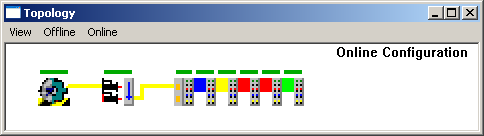
\includegraphics[width=0.95\textwidth]{images/topologyCP} \caption{Topologia stanowiska typu CP.} \label{topology:cp} \end{figure}
%\begin{figure}[!htb] 	\centering 	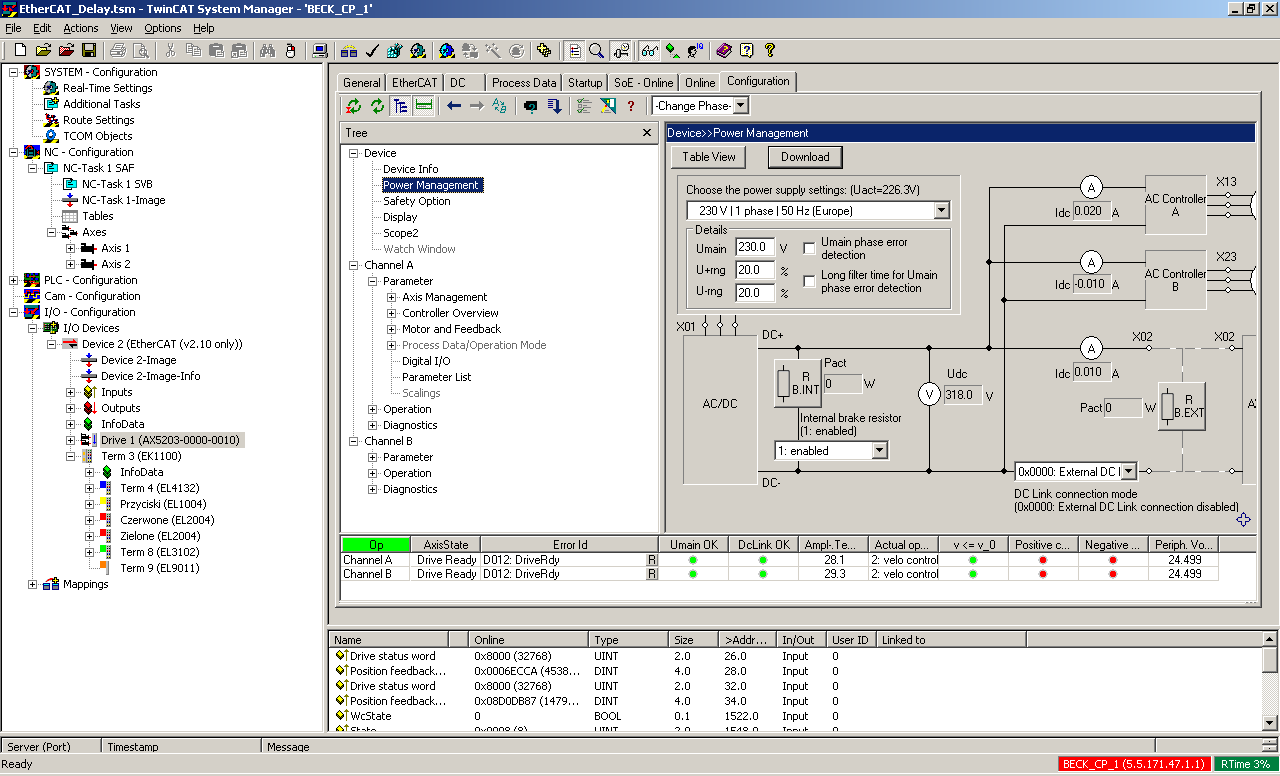
\includegraphics[width=0.99\textwidth]{images/confCP} \caption{Konfiguracja stanowiska typu CP} \label{conf:cp} \end{figure}

Na zrzucie ekranu dla stanowiska typu CP zauważyć można, że do węzła z~uruchomionym oprogramowaniem TwinCAT (ikona w~lewej części okna; w~tym przypadku sterownika~PLC) za pomocą ekranowanej skrętki (żółte połączenie na rysunku) został podłączony napęd serwomechanizmów, a~dopiero do niego za pomocą tego samego medium transmisyjnego zdalny zestaw modułów I/O. Podgląd topologii niestety nie uwzględnia połączenia pomiędzy elementami składowymi wyspy, które jest zrealizowane z~wykorzystaniem łącza E-bus. Moduły przylegają bezpośrednio do siebie, co jest zgodne ze stanem fizycznym, ale zdaniem autora połączenie takie powinno być w~pewien sposób zobrazowane, ponieważ osoba nie znająca dobrze protokołu, w tym szczególnie studenci na zajęciach laboratoryjnych mogą nie być świadomi, że są to osobne węzły sieci EtherCAT.
\clearpage
%\begin{figure}[!htb] 	\centering 	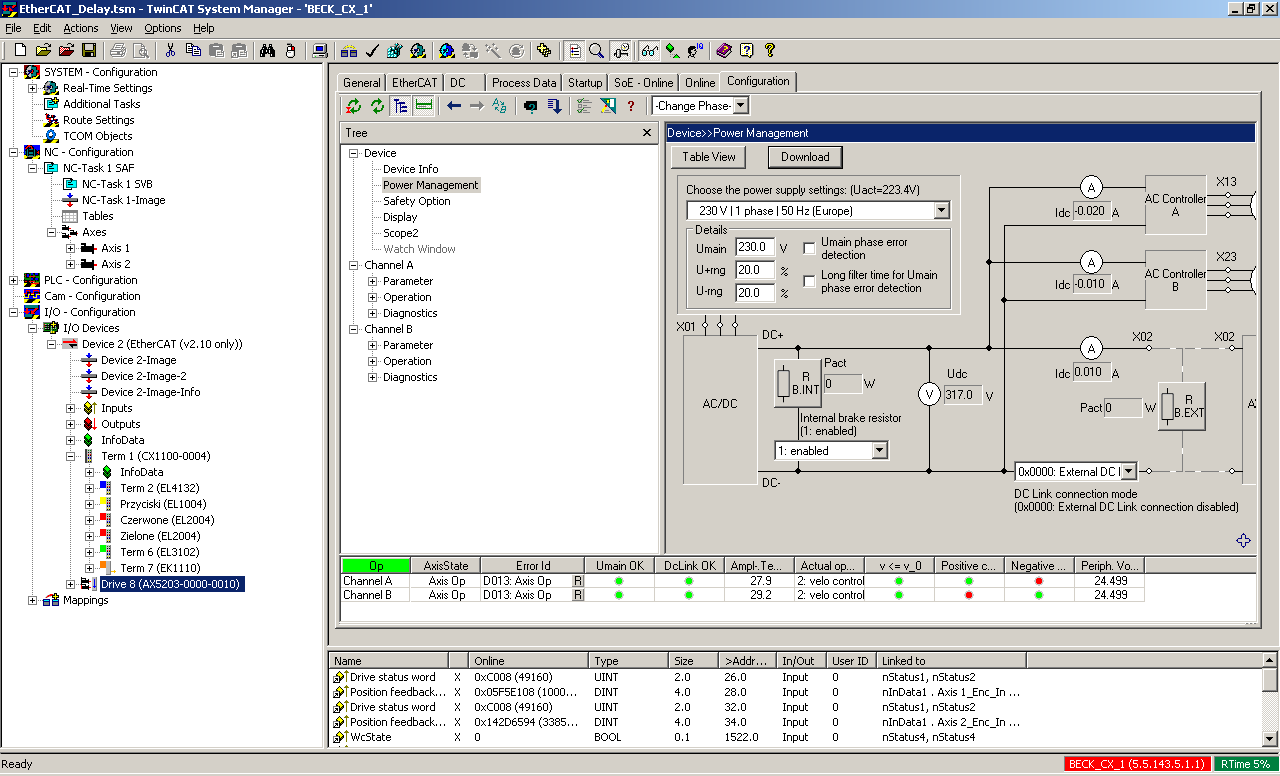
\includegraphics[width=0.99\textwidth]{images/confCX} \caption{Konfiguracja stanowiska typu CX} \label{conf:cx} \end{figure}
\begin{figure}[!htb] 	\centering 	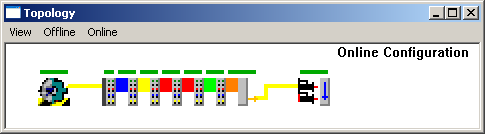
\includegraphics[width=0.95\textwidth]{images/topologyCX} \caption{Topologia stanowiska typu CX.} \label{topology:cx} \end{figure}

Topologia stanowiska typu CX różni się zasadniczo tylko kolejnością węzłów. Moduły wejścia/wyjścia są tutaj podłączone do jednostki centralnej protokołem EtherCAT w~oparciu o~łącze E-bus. Ostatnim tak podłączonym elementem jest terminal przyłączeniowy EK1100, do którego za pomocą kabla miedzianego (żółte połączenie na rysunku) podłączony jest napęd serwomechanizmów. W~przypadku tej topologii niezrozumiałe jest dla autora wprowadzenie żółtego połączenia pomiędzy jednostką centralną, a~pierwszym modułem, ponieważ jest to niekonsekwentne oraz sugeruje, że w~tym miejscu występuje połączenie kablem miedzianym.

Głównym problemem związanym z~uruchomieniem pełnych możliwości stanowisk było prawidłowe skonfigurowanie oraz uruchomienie serwomechanizmów napędzanych przez moduł~AX5203, co zostanie szczegółowo opisane w podrozdziale~\ref{subsec:problemy}.

Zgodnie z~założeniami należało przygotować oprogramowanie sterownika~PLC oraz wizualizację umożliwiającą obserwację zależności czasowych występujących w~protokole EtherCAT. Autor próbował znaleźć w~standardowych bibliotekach timer umożliwiający zmierzenie czasu trwania stanu wysokiego sygnału dyskretnego. Niestety wszystkie dostępne w~środowisku zegary samoczynnie resetowały zmierzoną wartość czasu po zakończeniu odmierzania. Z~tego powodu autor zdecydował się na własną implementację stopera. Kod stworzonego bloku funkcyjnego przedstawiono na Listingu~\ref{stopwatch_source}. Stoper jest uruchamiany w~momencie pojawienia się wartości \textit{TRUE} na wejściu \textit{start\_stop} i~odmierza czas aż do ponownej zmiany na wartość \textit{FALSE}. Bezpośrednio przed zatrzymaniem stopera odmierzona wartość jest przepisywana do zmiennej wyjściowej, dodatkowo w~czasie pracy stoper na bieżąco przepisuje zmierzoną wartość do zmiennej wyjściowej. Zdaniem autora tak stworzony stoper można określić jako stoper z~pamięcią. Przykładowa definicja i~zastosowanie stopera zostały przedstawione w~Listingu~\ref{stopwatch_using}.
\clearpage
\begin{lstlisting}[caption={Kod źródłowy stopera.},label=stopwatch_source]
FUNCTION_BLOCK STOPWATCH
VAR_INPUT
	max_value: TIME:=t#10S;
	start_stop: BOOL := FALSE;
END_VAR
VAR_OUTPUT
	value: TIME := t#0s;
END_VAR
VAR
	timer: TON;
END_VAR

IF timer.PT <> max_value THEN
	timer.PT := max_value;
END_IF;

IF start_stop = TRUE THEN
	timer(IN:=TRUE);
	value :=timer.ET;
ELSE
	IF timer.IN THEN
		value :=timer.ET;
	END_IF;
	timer(IN:=FALSE);
END_IF;
\end{lstlisting}

\begin{lstlisting}[caption={Wywołania odmierzania czasu stworzonym \\ blokiem funkcyjnym \textit{STOPWATCH}.},label=stopwatch_using]
PROGRAM MAIN
VAR
	stoper_device8: STOPWATCH := (max_value:=t#20s);
	stoper_axis1: STOPWATCH := (max_value:=t#120s);
END_VAR	
...
stoper_device8.start_stop := state_device8 <> 8;
stoper_device8();

stoper_axis1.start_stop := NOT axis1_Not_moving;
stoper_axis1();
\end{lstlisting}

Po skonfigurowaniu stanowiska oraz po stworzeniu odpowiedniego oprogramowania ostatnim elementem do przygotowania była wizualizacja. Widok projektu przygotowanej wizualizacji został przedstawiony na Rysunku~\ref{vis_szablon}.
\begin{figure}[!htb] 	\centering 	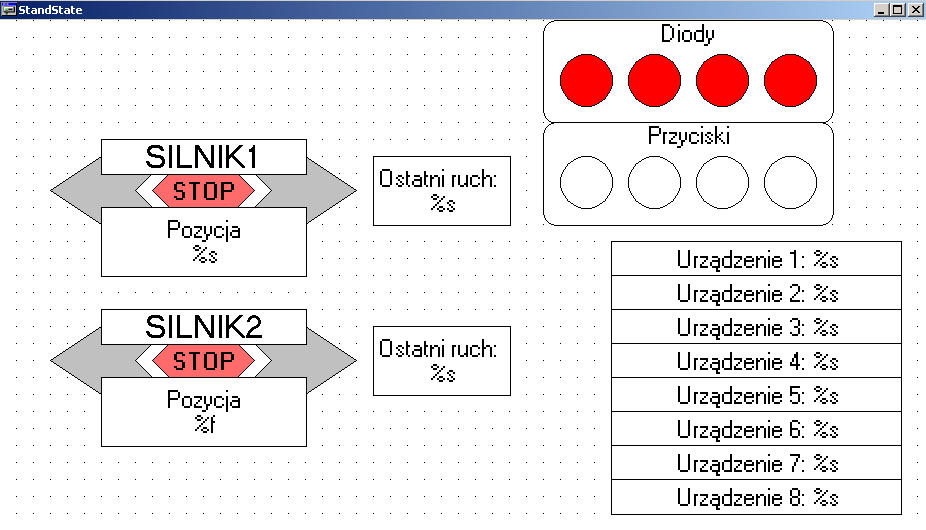
\includegraphics[width=0.99\textwidth]{images/vis_szablon} \caption{Projekt wizualizacji.} \label{vis_szablon} \end{figure}

Podstawowym elementem jest przedstawienie stanu najważniejszych urządzeń wejściowych i~wyjściowych. W~górnej części znajdują się elementy odwzorowujące stan diod LED oraz przycisków monostabilnych. Prawa strona przedstawia stan obu silników, a~dokładnie, czy są one w~ruchu oraz w którym kierunku. Dodatkowo została umieszczona informacja z~enkodera o~aktualnej pozycji silnika. W~celu przystosowania wizualizacji do obserwowania czasów mierzonych przez autora w~swoich badaniach została ona uzupełniona o~wartości mierzone za pomocą stworzonego stopera. 
\noindent Przykładowy wygląd stworzonej wizualizacji w~czasie pomiarów został przedstawiony na Rysunku~\ref{vis_inuse}.

\noindent Na ekranie można zaobserwować stan początkowy stanowiska po uruchomieniu. Silniki są ustawione na pozycjach 0, stan pracy żadnego z węzłów nie był zaburzany oraz naciśnięto 3~przyciski, co poskutkowało wyłączeniem diod czerwonych i~załączeniem diod zielonych.
\clearpage
\begin{figure}[!htb] 	\centering 	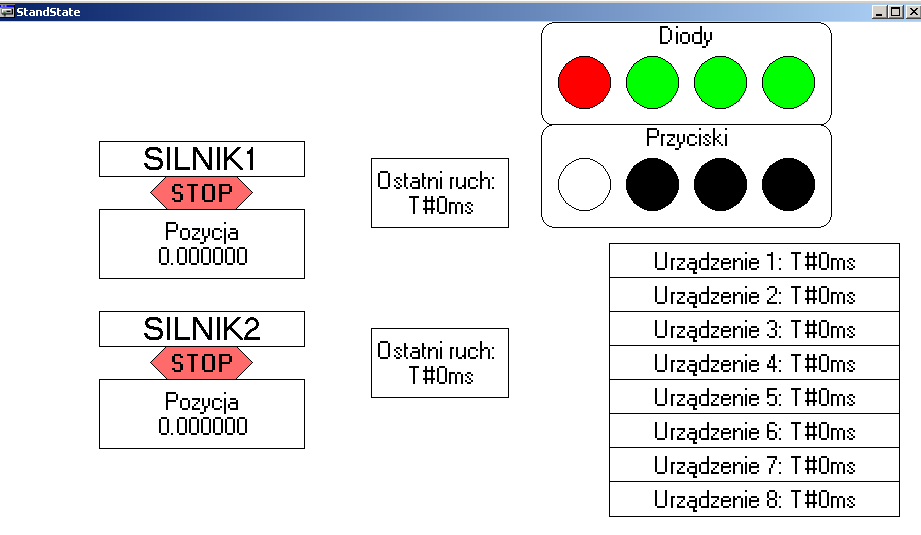
\includegraphics[width=0.99\textwidth]{images/vis_inuse2} \caption{Przykładowa uruchomiona wizualizacja.} \label{vis_inuse} \end{figure}
\vspace{-15mm}
\subsection{Rozbudowane stanowisko}
Stanowisko to posłuży do zbadania, jaki wpływ na wcześniejsze eksperymenty ma zwiększenie liczby węzłów. Liczba wszystkich węzłów podrzędnych wynosi 15 i~jest to maksymalna ilość jaką można uzyskać na dwóch wykorzystywanych stanowiskach. Uzyskana topologia rozbudowanego stanowiska została przedstawiona na Rysunku~\ref{topology:cx++}.
Na przedstawionym zrzucie ekranu widać, że podstawą do stworzenia rozszerzonej wersji było stanowisko CX z~podłączonymi za pomocą łącza E-bus modułami wejścia/wyjścia. Do zestawu tego, za pomocą kabla miedzianego (żółte połączenia na rysunku), zostały podłączone kolejno: zdalne moduły wejścia/wyjścia, pierwszy napęd serwomechanizmów oraz na końcu drugi napęd.

\begin{figure}[!htb] 	\centering 	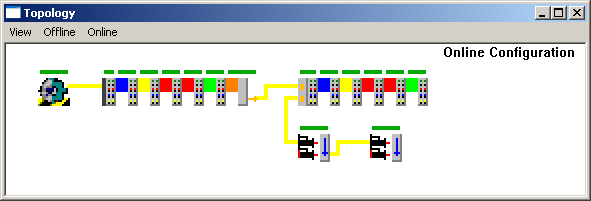
\includegraphics[width=0.95\textwidth]{images/topologyCX++} \caption{Topologia stanowiska typu CX++.} \label{topology:cx++} \end{figure}

Na tak przygotowanym stanowisku, w~celu uniknięcia różnic powstałych przez zastosowane oprogramowanie sterownika~PLC, autor zdecydował się uruchomić projekt przygotowany dla wersji podstawowej. Wybrane zostały po dwa przyciski, diody czerwone oraz diody zielone z~każdego stanowiska. Celem przeprowadzenia eksperymentów związanych z~opóźnieniem transmisji do wizualizacji i~oprogramowania zostały przypisane silniki, których automatyczne wykrycie udostępnia środowisko do zarządzania projektem.

Na rozbudowanym już stanowisku autor postanowił zrealizować drugą koncepcję pomiaru zależności czasowych w~protokole EtherCAT. Pomysłem było stworzenie oprogramowania umożliwiającego ruch silnika przez zadany czas. Stworzone wcześniej oprogramowanie zostało rozszerzone o~warunek zezwolenia na ruch silnika. Tak jak poprzednio stoper jest wyzwalany uruchomieniem silnika, a w tym przypadku sygnał \textit{Q} pochodzący z~timera znajdującego się wewnątrz bloku funkcyjnego \textit{STOPWATCH} (aktywowany w~momencie odmierzenia zadanego czasu) posłużył do cofnięcia zezwolenia na ruch. Zmodyfikowany kod źródłowy został przedstawiony w~Listingu~\ref{servoDist}.

\vspace{5mm}
\begin{lstlisting}[caption={Oprogramowanie odmierzające drogę przebytą w zadanym czasie.},label=servoDist]
PROGRAM MAIN
VAR
	stoper_axis1: STOPWATCH := (max_value:=t#120s);
	stoper_axis2: STOPWATCH := (max_value:=t#120s);
END_VAR

Enable_1 := NOT stoper_axis1.timer.Q;
Enable_2 := NOT stoper_axis2.timer.Q;

stoper_axis1.start_stop := NOT axis1_Not_moving;
stoper_axis1();
axis1_driving_time := stoper_axis1.value;
stoper_axis2.start_stop := NOT axis2_Not_moving;
stoper_axis2();
axis2_driving_time := stoper_axis2.value;
\end{lstlisting}

\clearpage
Decydując się na zmianę oprogramowania sterownika autor postanowił zmodyfikować również wizualizację. Przede wszystkim usunięto z~niej elementy związane z~pomiarem czasu stabilizacji stanu urządzeń. Dodatkowo umieszczono na niej informację o~aktualnej prędkość silnika.
Stworzoną wizualizacje typu drugiego przedstawiono na Rysunku~\ref{vis2_inuse}.
\begin{figure}[!htb] 	\centering 	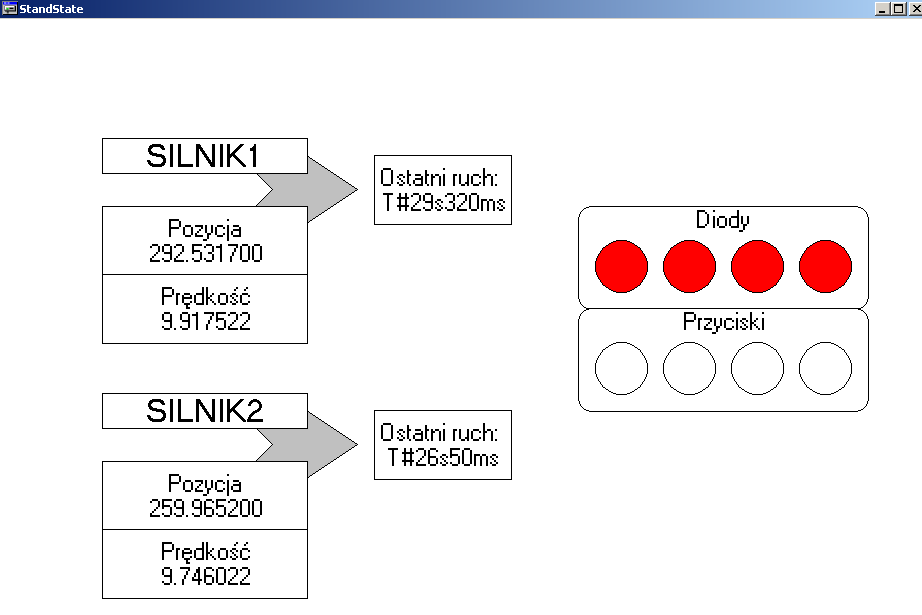
\includegraphics[width=0.99\textwidth]{images/vis2_inuse} \caption{Przykładowa uruchomiona wizualizacja typu drugiego.} \label{vis2_inuse} \end{figure}

Tak przygotowany kod sterownika PLC oraz wizualizacja posłużyły do przeprowadzenia badania drogi przebytej przez silnik w zdanym czasie, ze stałą prędkością. 
%ToDo: topologia, poprawić opis, jak zastosować istniejący kod i wizualizację do badań.
%\subsection{Opóźnienia pojedynczego odcinka sieci}
%\subsection{Wpływ topologi na opóźnienia}
%\subsection{Czas stabilizacji sieci po zmianach}
%
%Różne kable
%Długość kabla
%

%Połączyć do jednego sterownika oba napędy kolejno i zrobić coś na zasadzie inkrementacji i sprawdzić czy się przypadkiem nie rozjedzie
%
%Mamy opóźnienie na jednym odcinku
%
%Ewentualnie jeden kabel można zamienić na dłuższy i sprawdzić czy nie ma różnicy.
%
%Wymyślić jak sprawdzić czas ponownego włączenia do sieci.